\documentclass[aspectratio=169]{beamer}
%\usetheme{CambridgeUS}
%\usecolortheme{beaver}

%\usefonttheme{serif}
%\usepackage{helvet}

\usefonttheme{serif}     % Font theme: serif
%\usepackage{ccfonts}     % Font family: Concrete Math
\usepackage[T1]{fontenc} % Font encoding: T1

\setbeamersize{text margin left=42pt,text margin right=42pt} 
\setbeamertemplate{navigation symbols}{}
\setbeamertemplate{itemize items}[default]

\beamertemplatenavigationsymbolsempty

\definecolor{fore}{RGB}{51,51,51}
\definecolor{back}{RGB}{255, 254, 250}
\definecolor{title}{RGB}{ 255, 15, 0}
\definecolor{links}{RGB}{18, 168, 255}

\setbeamercolor{titlelike}{fg=title}
\setbeamercolor{normal text}{fg=fore,bg=back}
\setbeamercolor{alerted text}{fg=title}
\setbeamercolor{itemize item}{fg=title}
\setbeamercolor{enumerate item}{fg=title}
\hypersetup{colorlinks,urlcolor=links}

% for code https://kbroman.org/blog/2013/10/07/better-looking-latexbeamer-slides/
\usepackage{listings}
\definecolor{keywords}{RGB}{255,0,90}
\definecolor{comments}{RGB}{60,179,113}
\lstset{language=Python,
keywordstyle=color{keywords},
commentstyle=color{comments}emph}

% fonts
\usepackage[sc]{mathpazo}


% title info
\title{\textbf{Transportation Planning \& Decision-Making}
\subtitle{\textbf{GGR424 - Transportation Geography \& Planning}}
\author{Jeff Allen}
\institute{University of Toronto}
\date{March 14, 2022}}




\begin{document}
	
\begin{frame}
	\titlepage	
\end{frame}





\begin{frame}
	
	\textbf{Announcements}
	
	\begin{itemize}
		\item Presentations on March 28 and April 4, message me if you have a date preference 
	\end{itemize}
	
	
	\textbf{Today}
	
	\begin{itemize}
		\item Finish up material on equity from last week
		\item Transit planning activity
		
	\end{itemize}
\end{frame}




\begin{frame}
	
	\textbf{Cost-Benefit Analysis}
	
	\begin{itemize}
		\item Compares the pros and cons of different transportation policy and planning options, to aid decision-making
		\item Usually by converting metrics (e.g. emissions, travel time savings) into dollars
		
		\tiny\url{https://vtpi.org/tca/}
	\end{itemize}	
	
	\textbf{Business Case}
	
	\begin{itemize}
		\item "comprehensive
		collection of evidence and analysis
		that sets out the rationale for why an
		investment should be implemented" - Metrolinx
		
		\tiny\url{https://www.metrolinx.com/en/regionalplanning/projectevaluation/benefitscases/benefits_case_analyses.aspx}
	\end{itemize}
	
\end{frame}




\begin{frame}
	
	\textbf{5 Transit lines undergoing planning and design in Toronto:}
	
	\begin{itemize}
		\item Eglinton East
		\item Eglinton West
		\item Ontario Line
		\item Scarborough Subway Extension
		\item Yonge Subway Extension
	\end{itemize}
	
	\textbf{In your group}
	
	\begin{enumerate}
		\item Provide a background on the project / route
		\item Look at at least 2 design options for improvement
		\item Create an evaluation table, comparing the options
		\item Present findings and make a recommendation
	\end{enumerate}

	\url{https://docs.google.com/presentation/d/1opoNq3CNhyuVkiRQOSOHFFnxcojo0UqWIosWqha9Ri8/edit?usp=sharing}
	
\end{frame}



\begin{frame}
	
	e.g. Evaluation table
	
	\begin{figure}
		\centering
		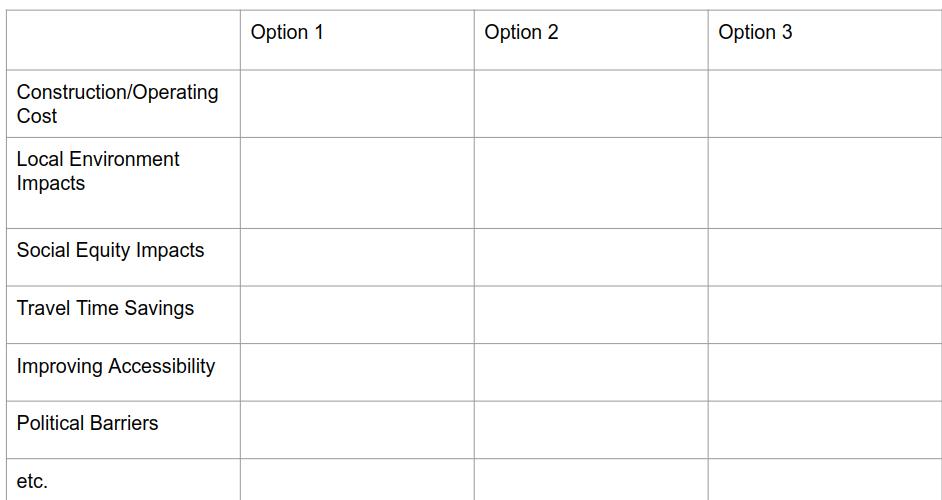
\includegraphics[width=1\linewidth]{images/evaluation_table.png}
	\end{figure}
	
\end{frame}








\end{document}